%{{{
%\documentclass{scrartcl}
%\usepackage{tikz}
%\usetikzlibrary{arrows,automata,tikz-timing}
%
%\begin{document}
%\resizebox{\linewidth}{!}{%
%	\centering
%\begin{tikzpicture}[>=stealth',shorten >=1pt,auto,node distance=2cm]
%	\node[initial,state,accepting] (idl_rdtg)                                          {$idl\_rdtg$};
%	\node[state]                   (cmp_dlv)  [right of=idl_rdtg, node distance=7.0cm] {$cmp\_dlv$};
%	\node[state]                   (rq0)      [right of=cmp_dlv,  node distance=7.0cm] {$rq_0$};
%	\node[state]                   (rq1)      [below of=rq0,      node distance=4.5cm] {$rq_1$};
%	\node[state]                   (rd0)      [below of=rq1,      node distance=4.5cm] {$rd_0$};
%	\node[state]                   (rd1)      [left  of=rd0]                           {$rd_1$};
%	\node[state]                   (rd1_)     [above of=rd1]                           {$rd_1'$};
%	\node[state]                   (rd2)      [left  of=rd1]                           {$rd_2$};
%	\node[state]                   (rd3)      [left  of=rd2]                           {$rd_3$};
%	\node[state]                   (rd4)      [left  of=rd3]                           {$rd_4$};
%	\node[state]                   (rd5)      [left  of=rd4]                           {$rd_5$};
%	\node[state]                   (rd6)      [left  of=rd5]                           {$rd_6$};
%	\node[state]                   (rd7)      [left  of=rd6]                           {$rd_7$};
%	\node[state]                   (wait)     [above of=rd7,      node distance=4.5cm] {$wait$};
%
%
%	\path[->] (idl_rdtg)  edge [loop above] node {a} (idl_rdtgS)
%	                      edge [bend left]  node {a} (cmp_dlv)
%	          (cmp_dlv)   edge              node {a} (idl_rdtg)
%	                      edge              node {b} (rq0)
%	                      edge              node {b} (rq1)
%						  edge [bend left]  node {b} (rd0)
%	          (rq0)       edge [loop above] node {b} (rq0)
%	                      edge              node {b} (rq1)
%	                      edge [bend left]  node {X} (rd0)
%
%
%
%
%						  ;
%\end{tikzpicture}
%}
%
%
%
%\resizebox{\linewidth}{!}{%
%	\centering
%\begin{tikztimingtable}[%
%		timing/dslope=0.2,
%		timing/dslope=0.2,
%		%timing/name/.style={font=\sffamily\scriptsize},
%		%timing/d/text/.style={font=\sffamily\tiny},
%		%rayz/.style={timing/z/.append style={gray}},
%		%iming/n/.style={rectangle},
%		timing/metachar={{K}[2]{#1h!{++(0,-.5\yunit)} N[rectangle,scale=.3]{#2}!{++(0,+.5\yunit)} #1h}},
%		timing/metachar={{J}[2]{#1l!{++(0,+.5\yunit)} N[rectangle,scale=.3]{#2}!{++(0,-.5\yunit)} #1l}},
%	]
%	SDA$_{Master}$ & hL DD{A}{} d[dotted]D;d{}DD{A}{} HK{R}{} HH HH HH; h[dotted]H;h HH HH HK{NACK} LLhH \\
%	SDA$_{Slave}$  & hH HH     ;h[dotted]H;h  HH      HH        LJ{ACK} HH DD{D}{} d[dotted]D;d{}DD{D}{} DD{D}{} HK{} HHhH \\
%	SDA            & hL DD{A}{} d[dotted]D;d{}DD{A}{} HK{R}{} LJ{ACK} HH DD{D}{} d[dotted]D;d{}DD{D}{} DD{D}{} HK{NACK} LLhH \\
%	SCL & HLK{1} L;  [dotted]L;L   K{7} L  K{8} L    K{9}   LL LK{1} L; [dotted]L;L   K{7} L  K{8} L  K{9}   LLHH \\
%	\extracode
%	\begin{background}
%		\vertlines[help lines]{}
%		\horlines[help lines]{}
%		\show\horlines
%	%	\draw [->,>=latex] (0,-\nrows-1) -- (\twidth+1,-\nrows-1);
%	%	\foreach \n in {0,1,...,\twidth}
%	%	\draw (\n,-\nrows-1+.1) -- +(0,-.2)
%	%	node [below,inner sep=2pt] {\scalebox{.75}{\tiny\n}};
%	\end{background}
%	%\tablegrid[black!25]
%\end{tikztimingtable}
%}
%
%\end{document}
%}}}




\documentclass[12pt]{article}
\usepackage{tikz}

\begin{document}

\resizebox{\linewidth}{!}{%
	\centering
%\begin{center}
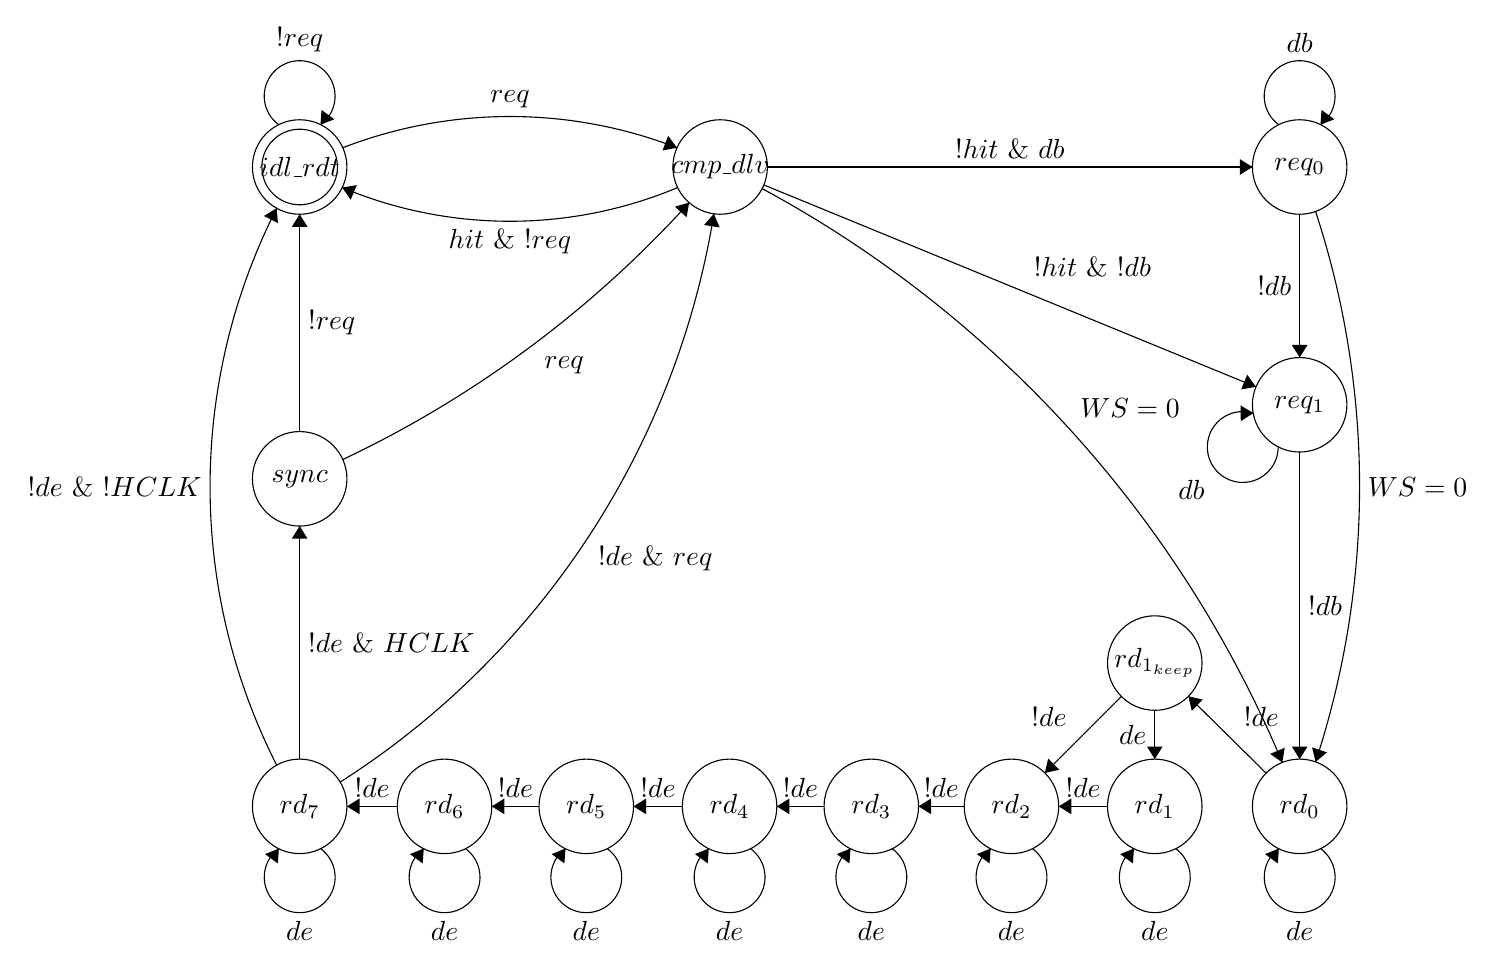
\begin{tikzpicture}[scale=0.2]
\tikzstyle{every node}+=[inner sep=0pt]
\draw [black] (13.1,-9.8) circle (3);
\draw (13.1,-9.8) node {$idl\_rdt$};
\draw [black] (13.1,-9.8) circle (2.4);
\draw [black] (39.8,-9.8) circle (3);
\draw (39.8,-9.8) node {$cmp\_dlv$};
\draw [black] (76.6,-24.9) circle (3);
\draw (76.6,-24.9) node {$req_1$};
\draw [black] (76.6,-50.4) circle (3);
\draw (76.6,-50.4) node {$rd_0$};
\draw [black] (67.4,-50.4) circle (3);
\draw (67.4,-50.4) node {$rd_1$};
\draw [black] (58.3,-50.4) circle (3);
\draw (58.3,-50.4) node {$rd_2$};
\draw [black] (49.4,-50.4) circle (3);
\draw (49.4,-50.4) node {$rd_3$};
\draw [black] (40.4,-50.4) circle (3);
\draw (40.4,-50.4) node {$rd_4$};
\draw [black] (31.3,-50.4) circle (3);
\draw (31.3,-50.4) node {$rd_5$};
\draw [black] (22.3,-50.4) circle (3);
\draw (22.3,-50.4) node {$rd_6$};
\draw [black] (13.1,-50.4) circle (3);
\draw (13.1,-50.4) node {$rd_7$};
\draw [black] (13.1,-29.6) circle (3);
\draw (13.1,-29.6) node {$sync$};
\draw [black] (76.6,-9.8) circle (3);
\draw (76.6,-9.8) node {$req_0$};
\draw [black] (67.4,-41.3) circle (3);
\draw (67.4,-41.3) node {$rd_{1_{keep}}$};
\draw [black] (15.838,-8.576) arc (111.1609:68.8391:29.398);
\fill [black] (37.06,-8.58) -- (36.5,-7.82) -- (36.14,-8.75);
\draw (26.45,-6.09) node [above] {$req$};
\draw [black] (76.6,-27.9) -- (76.6,-47.4);
\fill [black] (76.6,-47.4) -- (77.1,-46.6) -- (76.1,-46.6);
\draw (77.1,-37.65) node [right] {$!db$};
\draw [black] (55.3,-50.4) -- (52.4,-50.4);
\fill [black] (52.4,-50.4) -- (53.2,-50.9) -- (53.2,-49.9);
\draw (53.85,-49.9) node [above] {$!de$};
\draw [black] (46.4,-50.4) -- (43.4,-50.4);
\fill [black] (43.4,-50.4) -- (44.2,-50.9) -- (44.2,-49.9);
\draw (44.9,-49.9) node [above] {$!de$};
\draw [black] (37.4,-50.4) -- (34.3,-50.4);
\fill [black] (34.3,-50.4) -- (35.1,-50.9) -- (35.1,-49.9);
\draw (35.85,-49.9) node [above] {$!de$};
\draw [black] (28.3,-50.4) -- (25.3,-50.4);
\fill [black] (25.3,-50.4) -- (26.1,-50.9) -- (26.1,-49.9);
\draw (26.8,-49.9) node [above] {$!de$};
\draw [black] (19.3,-50.4) -- (16.1,-50.4);
\fill [black] (16.1,-50.4) -- (16.9,-50.9) -- (16.9,-49.9);
\draw (17.7,-49.9) node [above] {$!de$};
\draw [black] (13.1,-47.4) -- (13.1,-32.6);
\fill [black] (13.1,-32.6) -- (12.6,-33.4) -- (13.6,-33.4);
\draw (13.6,-40) node [right] {$!de\mbox{ }\&\mbox{ }HCLK$};
\draw [black] (13.1,-26.6) -- (13.1,-12.8);
\fill [black] (13.1,-12.8) -- (12.6,-13.6) -- (13.6,-13.6);
\draw (13.6,-19.7) node [right] {$!req$};
\draw [black] (11.777,-7.12) arc (234:-54:2.25);
\draw (13.1,-2.55) node [above] {$!req$};
\fill [black] (14.42,-7.12) -- (15.3,-6.77) -- (14.49,-6.18);
\draw [black] (75.235,-27.558) arc (0.54782:-287.45218:2.25);
\draw (70.6,-30.31) node [left] {$db$};
\fill [black] (73.66,-25.43) -- (72.85,-24.94) -- (72.86,-25.94);
\draw [black] (77.923,-53.08) arc (54:-234:2.25);
\draw (76.6,-57.65) node [below] {$de$};
\fill [black] (75.28,-53.08) -- (74.4,-53.43) -- (75.21,-54.02);
\draw [black] (68.723,-53.08) arc (54:-234:2.25);
\draw (67.4,-57.65) node [below] {$de$};
\fill [black] (66.08,-53.08) -- (65.2,-53.43) -- (66.01,-54.02);
\draw [black] (59.623,-53.08) arc (54:-234:2.25);
\draw (58.3,-57.65) node [below] {$de$};
\fill [black] (56.98,-53.08) -- (56.1,-53.43) -- (56.91,-54.02);
\draw [black] (50.723,-53.08) arc (54:-234:2.25);
\draw (49.4,-57.65) node [below] {$de$};
\fill [black] (48.08,-53.08) -- (47.2,-53.43) -- (48.01,-54.02);
\draw [black] (41.723,-53.08) arc (54:-234:2.25);
\draw (40.4,-57.65) node [below] {$de$};
\fill [black] (39.08,-53.08) -- (38.2,-53.43) -- (39.01,-54.02);
\draw [black] (32.623,-53.08) arc (54:-234:2.25);
\draw (31.3,-57.65) node [below] {$de$};
\fill [black] (29.98,-53.08) -- (29.1,-53.43) -- (29.91,-54.02);
\draw [black] (23.623,-53.08) arc (54:-234:2.25);
\draw (22.3,-57.65) node [below] {$de$};
\fill [black] (20.98,-53.08) -- (20.1,-53.43) -- (20.91,-54.02);
\draw [black] (14.423,-53.08) arc (54:-234:2.25);
\draw (13.1,-57.65) node [below] {$de$};
\fill [black] (11.78,-53.08) -- (10.9,-53.43) -- (11.71,-54.02);
\draw [black] (37.833,-12.065) arc (-42.20032:-64.68041:70.24);
\fill [black] (37.83,-12.06) -- (36.93,-12.32) -- (37.67,-12.99);
\draw (29.89,-21.8) node [below] {$req$};
\draw [black] (39.405,-12.773) arc (-9.19845:-57.46223:52.82);
\fill [black] (39.4,-12.77) -- (38.78,-13.48) -- (39.77,-13.64);
\draw (32.01,-34.68) node [right] {$!de\mbox{ }\&\mbox{ }req$};
\draw [black] (37.101,-11.107) arc (-67.284:-112.716:27.582);
\fill [black] (15.8,-11.11) -- (16.34,-11.88) -- (16.73,-10.95);
\draw (26.45,-13.75) node [below] {$hit\mbox{ }\&\mbox{ }!req$};
\draw [black] (64.4,-50.4) -- (61.3,-50.4);
\fill [black] (61.3,-50.4) -- (62.1,-50.9) -- (62.1,-49.9);
\draw (62.85,-49.9) node [above] {$!de$};
\draw [black] (76.6,-12.8) -- (76.6,-21.9);
\fill [black] (76.6,-21.9) -- (77.1,-21.1) -- (76.1,-21.1);
\draw (76.1,-17.35) node [left] {$!db$};
\draw [black] (42.58,-10.94) -- (73.82,-23.76);
\fill [black] (73.82,-23.76) -- (73.27,-22.99) -- (72.89,-23.92);
\draw (63.44,-16.76) node [above] {$!hit\mbox{ }\&\mbox{ }!db$};
\draw [black] (75.277,-7.12) arc (234:-54:2.25);
\draw (76.6,-2.55) node [above] {$db$};
\fill [black] (77.92,-7.12) -- (78.8,-6.77) -- (77.99,-6.18);
\draw [black] (42.8,-9.8) -- (73.6,-9.8);
\fill [black] (73.6,-9.8) -- (72.8,-9.3) -- (72.8,-10.3);
\draw (58.2,-9.3) node [above] {$!hit\mbox{ }\&\mbox{ }db$};
\draw [black] (11.64,-47.78) arc (-153.07961:-206.92039:39.05);
\fill [black] (11.64,-12.42) -- (10.83,-12.91) -- (11.72,-13.36);
\draw (6.91,-30.1) node [left] {$!de\mbox{ }\&\mbox{ }!HCLK$};
\draw [black] (74.47,-48.29) -- (69.53,-43.41);
\fill [black] (69.53,-43.41) -- (69.75,-44.33) -- (70.45,-43.62);
\draw (74.17,-45.37) node [above] {$!de$};
\draw [black] (67.4,-44.3) -- (67.4,-47.4);
\fill [black] (67.4,-47.4) -- (67.9,-46.6) -- (66.9,-46.6);
\draw (66.9,-45.85) node [left] {$de$};
\draw [black] (65.28,-43.42) -- (60.42,-48.28);
\fill [black] (60.42,-48.28) -- (61.34,-48.07) -- (60.63,-47.36);
\draw (60.68,-45.37) node [above] {$!de$};
\draw [black] (77.611,-12.624) arc (18.1628:-18.1628:56.063);
\fill [black] (77.61,-47.58) -- (78.34,-46.97) -- (77.39,-46.66);
\draw (80.9,-30.1) node [right] {$WS=0$};
\draw [black] (42.468,-11.172) arc (61.617:22.76157:73.928);
\fill [black] (75.5,-47.61) -- (75.65,-46.68) -- (74.73,-47.07);
\draw (62.64,-25.11) node [right] {$WS=0$};
\end{tikzpicture}
%\end{center}
}

\vspace*{1cm}
\begin{tabular}{l | l}
	Name & Description\\
	\hline
	req & HSEL \&\& !HRWITE \&\& HREADY \\
	hit & (TAGSRAM\_output[TAG] == SAVE0\_HADDR) \&\& TAGSRAM\_output[VALID]\\
	db  & baz\\
	de  & foobar\\
	WS  & adsf\\
\end{tabular}

\end{document}
